\documentclass[tikz,border=6pt]{standalone}
\usepackage{amsmath}
\usetikzlibrary{arrows.meta,positioning,fit,calc,backgrounds}

\definecolor{stageblue}{RGB}{53,114,190}
\definecolor{stageorange}{RGB}{230,132,54}
\definecolor{stagegreen}{RGB}{68,160,96}
\definecolor{stagered}{RGB}{196,74,74}
\definecolor{stagegray}{RGB}{110,110,110}
\definecolor{softblue}{RGB}{232,241,252}
\definecolor{softorange}{RGB}{253,239,226}
\definecolor{softgreen}{RGB}{231,247,236}
\definecolor{softred}{RGB}{252,236,236}
\definecolor{softgray}{RGB}{244,244,244}

\tikzset{
  >={Latex[length=2.0mm,width=1.5mm]},
  base/.style={draw=black!75, line width=0.35pt, rounded corners=2.2pt, align=left, font=\footnotesize, inner sep=2.8pt},
  stage/.style={base, fill=white},
  bluebox/.style={base, fill=softblue},
  orangebox/.style={base, fill=softorange},
  greenbox/.style={base, fill=softgreen},
  redbox/.style={base, fill=softred},
  graybox/.style={base, fill=softgray},
  title/.style={font=\bfseries\small, align=center},
  arrow/.style={-Latex, line width=0.45pt, draw=black!75},
  subtle/.style={font=\scriptsize, text=stagegray},
  emph/.style={font=\scriptsize\bfseries},
  mini/.style={font=\scriptsize, align=left}
}

\begin{document}
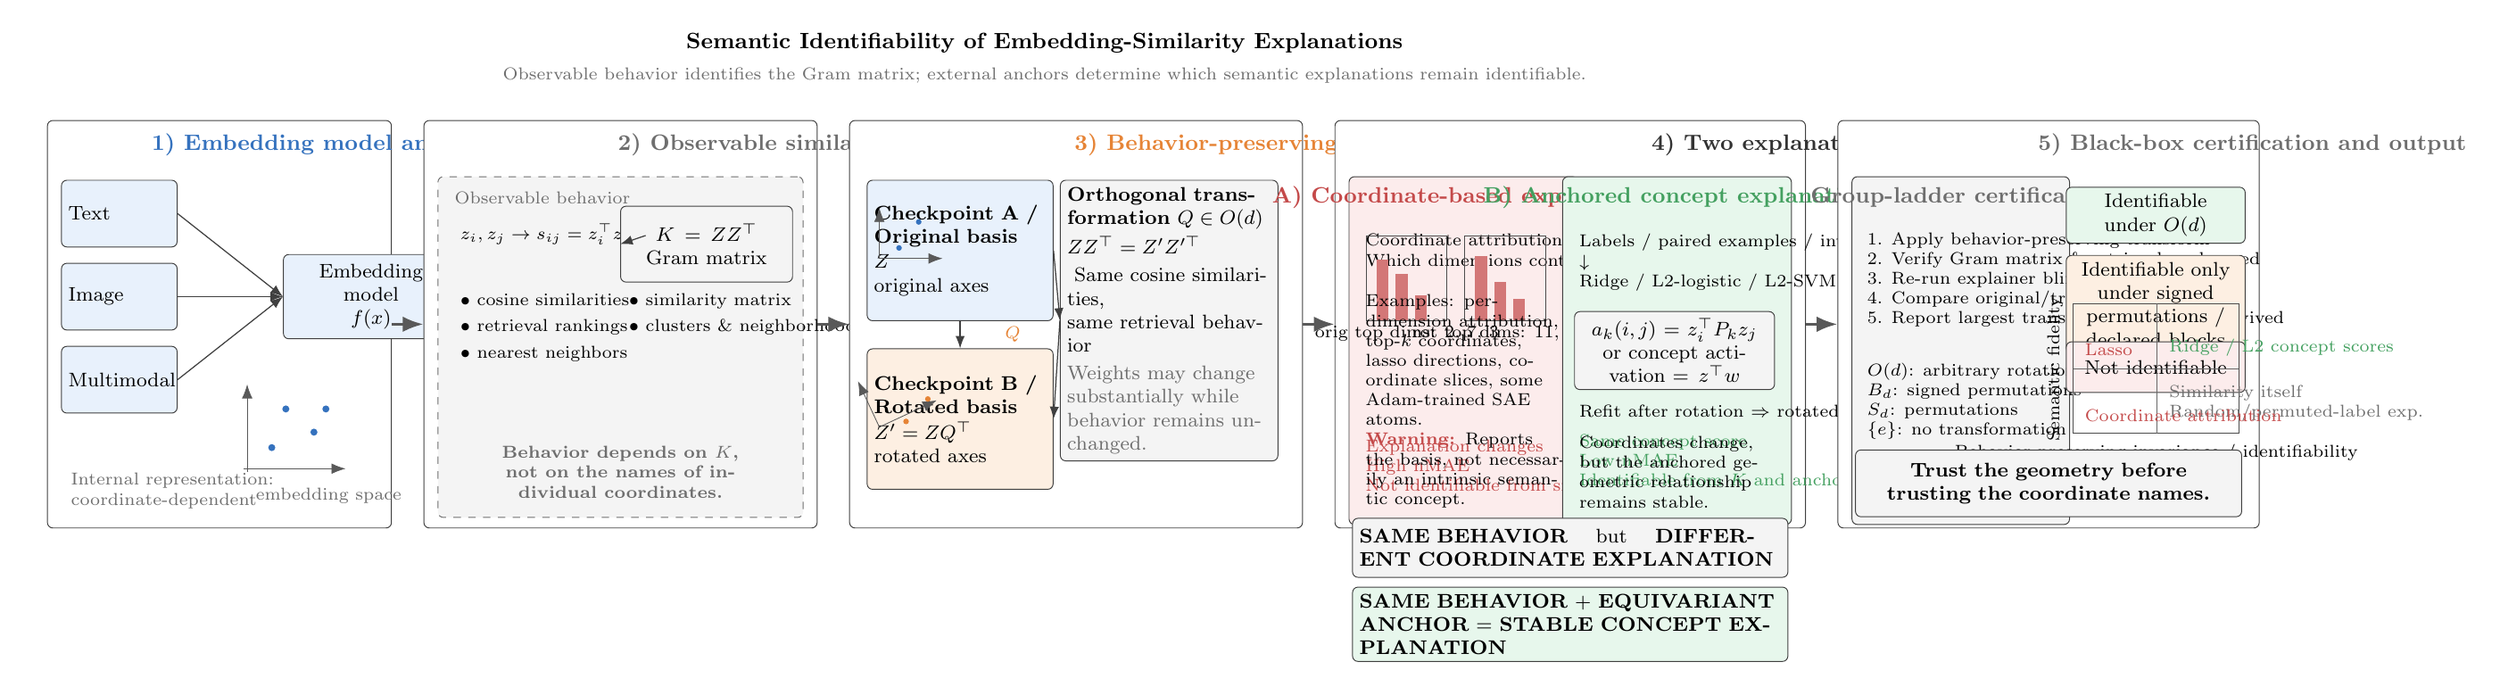
\begin{tikzpicture}[x=1cm,y=1cm]

% Header
\node[title, text width=28.8cm] (maintitle) at (14.4,9.05)
{Semantic Identifiability of Embedding-Similarity Explanations};
\node[subtle, text width=28.8cm, align=center] at (14.4,8.58)
{Observable behavior identifies the Gram matrix; external anchors determine which semantic explanations remain identifiable.};

% === Stage 1 ===
\node[stage, text width=4.7cm, minimum height=5.8cm, anchor=north west] (s1) at (0.2,7.95) {};
\node[title, text=stageblue] at ($(s1.north)+(2.35,-0.35)$) {1) Embedding model and representation};

\node[bluebox, text width=1.45cm, minimum height=0.95cm, anchor=north west] (in1) at ($(s1.north west)+(0.2,-0.85)$) {Text};
\node[bluebox, text width=1.45cm, minimum height=0.95cm, anchor=north west] (in2) at ($(in1.south west)+(0,-0.22)$) {Image};
\node[bluebox, text width=1.45cm, minimum height=0.95cm, anchor=north west] (in3) at ($(in2.south west)+(0,-0.22)$) {Multimodal};
\node[bluebox, text width=2.3cm, minimum height=1.2cm, anchor=west, align=center] (model) at ($(in2.east)+(1.5,0)$) {Embedding model\\$f(x)$};
\draw[arrow] (in1.east) -- (model.west);
\draw[arrow] (in2.east) -- (model.west);
\draw[arrow] (in3.east) -- (model.west);

\node[mini, text=stageblue, anchor=west] at ($(model.east)+(0.15,0.45)$) {$z=f(x)\in\mathbb{R}^d$};
\node[graybox, text width=1.85cm, minimum height=1.05cm, anchor=west, align=center] (zmat) at ($(model.east)+(0.2,-0.45)$) {$Z\in\mathbb{R}^{n\times d}$};
\draw[arrow] (model.east) -- ($(model.east)+(0.16,0)$);

\begin{scope}[shift={($(s1.south west)+(2.85,0.85)$)}]
  \draw[black!65, line width=0.3pt,->] (-0.05,0) -- (1.4,0);
  \draw[black!65, line width=0.3pt,->] (0,-0.05) -- (0,1.2);
  \fill[stageblue] (0.35,0.3) circle (0.05);
  \fill[stageblue] (0.55,0.85) circle (0.05);
  \fill[stageblue] (0.95,0.52) circle (0.05);
  \fill[stageblue] (1.12,0.85) circle (0.05);
  \node[subtle, anchor=north west] at (0,-0.15) {embedding space};
\end{scope}
\node[subtle, text width=4.2cm, anchor=south west] at ($(s1.south west)+(0.22,0.16)$)
{Internal representation: coordinate-dependent};

% === Stage 2 ===
\node[stage, text width=5.4cm, minimum height=5.8cm, anchor=north west] (s2) at ($(s1.north east)+(0.45,0)$) {};
\node[title, text=stagegray] at ($(s2.north)+(2.7,-0.35)$) {2) Observable similarity behavior};

\node[graybox, text width=5.0cm, minimum height=4.85cm, dashed, draw=stagegray, anchor=north west] (obs) at ($(s2.north west)+(0.2,-0.8)$) {};
\node[mini, text=stagegray, anchor=north west] at ($(obs.north west)+(0.12,-0.1)$) {Observable behavior};

\node[mini, anchor=north west] (zij) at ($(obs.north west)+(0.2,-0.55)$) {$z_i, z_j \rightarrow s_{ij}=z_i^\top z_j$};
\node[graybox, text width=2.25cm, minimum height=1.08cm, anchor=north west, align=center] (gram) at ($(obs.north west)+(2.6,-0.42)$) {$K=ZZ^\top$\\Gram matrix};
\draw[arrow] ($(zij.east)+(0.08,-0.02)$) -- (gram.west);

\node[mini, anchor=north west] at ($(obs.north west)+(0.2,-1.55)$) {$\bullet$ cosine similarities};
\node[mini, anchor=north west] at ($(obs.north west)+(0.2,-1.92)$) {$\bullet$ retrieval rankings};
\node[mini, anchor=north west] at ($(obs.north west)+(0.2,-2.29)$) {$\bullet$ nearest neighbors};
\node[mini, anchor=north west] at ($(obs.north west)+(2.6,-1.55)$) {$\bullet$ similarity matrix};
\node[mini, anchor=north west] at ($(obs.north west)+(2.6,-1.92)$) {$\bullet$ clusters \& neighborhoods};

\node[emph, text=stagegray, text width=4.72cm, align=center, anchor=south] at ($(obs.south)+(0,0.16)$)
{Behavior depends on $K$, not on the names of individual coordinates.};

% === Stage 3 ===
\node[stage, text width=6.25cm, minimum height=5.8cm, anchor=north west] (s3) at ($(s2.north east)+(0.45,0)$) {};
\node[title, text=stageorange] at ($(s3.north)+(3.13,-0.35)$) {3) Behavior-preserving transformation};

\node[bluebox, text width=2.45cm, minimum height=2.0cm, anchor=north west] (orig) at ($(s3.north west)+(0.25,-0.85)$)
{\textbf{Checkpoint A / Original basis}\\[0.08em]$Z$\\original axes};
\node[orangebox, text width=2.45cm, minimum height=2.0cm, anchor=south west] (rot) at ($(s3.south west)+(0.25,0.55)$)
{\textbf{Checkpoint B / Rotated basis}\\[0.08em]$Z'=ZQ^\top$\\rotated axes};
\node[graybox, text width=2.9cm, minimum height=2.9cm, anchor=north west] (eqv) at ($(s3.north west)+(3.0,-0.85)$)
{\textbf{Orthogonal transformation $Q\in O(d)$}\\[0.3em]
$ZZ^\top=Z'Z'^\top$\\[0.2em]
$\checkmark$ Same cosine similarities,\\same retrieval behavior\\[0.2em]
\textcolor{stagegray}{Weights may change substantially while behavior remains unchanged.}};

\draw[arrow] (orig.east) -- (eqv.west);
\draw[arrow] (eqv.west) -- (rot.east);
\draw[arrow] (orig.south) -- (rot.north);
\node[mini, text=stageorange] at ($(orig.south)!0.5!(rot.north)+(0.75,0)$) {$Q$};

\begin{scope}[shift={($(orig.north west)+(0.18,-1.12)$)}]
  \draw[black!65, line width=0.3pt,->] (0,0) -- (0.9,0);
  \draw[black!65, line width=0.3pt,->] (0,0) -- (0,0.72);
  \fill[stageblue] (0.28,0.15) circle (0.04);
  \fill[stageblue] (0.56,0.52) circle (0.04);
\end{scope}
\begin{scope}[shift={($(rot.north west)+(0.18,-1.12)$)}]
  \draw[black!65, line width=0.3pt,->,rotate around={25:(0,0)}] (0,0) -- (0.9,0);
  \draw[black!65, line width=0.3pt,->,rotate around={25:(0,0)}] (0,0) -- (0,0.72);
  \fill[stageorange] (0.38,0.08) circle (0.04);
  \fill[stageorange] (0.69,0.4) circle (0.04);
\end{scope}

% === Stage 4 ===
\node[stage, text width=6.5cm, minimum height=5.8cm, anchor=north west] (s4) at ($(s3.north east)+(0.45,0)$) {};
\node[title, text=black!80] at ($(s4.north)+(3.25,-0.35)$) {4) Two explanation types};

\node[redbox, text width=3.06cm, minimum height=4.95cm, anchor=north west] (coord) at ($(s4.north west)+(0.2,-0.8)$) {};
\node[title, text=stagered] at ($(coord.north)+(0,-0.3)$) {A) Coordinate-based explanation};
\node[mini, anchor=north west] at ($(coord.north west)+(0.12,-0.7)$)
{Coordinate attribution: $z_i\odot z_j$\\Which dimensions contributed?};

\begin{scope}[shift={($(coord.north west)+(0.25,-2.05)$)}]
  \draw[black!70, line width=0.25pt] (0,0) rectangle (1.15,1.2);
  \fill[stagered!75] (0.15,0) rectangle (0.32,0.86);
  \fill[stagered!75] (0.42,0) rectangle (0.59,0.66);
  \fill[stagered!75] (0.69,0) rectangle (0.86,0.36);
  \node[mini] at (0.58,-0.18) {orig top dims: 2, 7, 3};
\end{scope}
\begin{scope}[shift={($(coord.north west)+(1.65,-2.05)$)}]
  \draw[black!70, line width=0.25pt] (0,0) rectangle (1.15,1.2);
  \fill[stagered!75] (0.15,0) rectangle (0.32,0.92);
  \fill[stagered!75] (0.42,0) rectangle (0.59,0.55);
  \fill[stagered!75] (0.69,0) rectangle (0.86,0.31);
  \node[mini] at (0.58,-0.18) {rot top dims: 11, 4, 9};
\end{scope}
\node[mini, text=stagered, anchor=north west] at ($(coord.north west)+(0.12,-3.63)$)
{Explanation changes\\High nMAE\\Not identifiable from similarity behavior};
\node[mini, text width=2.86cm, anchor=south west] at ($(coord.south west)+(0.12,0.12)$)
{Examples: per-dimension attribution, top-$k$ coordinates, lasso directions, coordinate slices, some Adam-trained SAE atoms.\\\textbf{\textcolor{stagered}{Warning:}} Reports the basis, not necessarily an intrinsic semantic concept.};

\node[greenbox, text width=3.06cm, minimum height=4.95cm, anchor=north east] (anch) at ($(s4.north east)+(-0.2,-0.8)$) {};
\node[title, text=stagegreen] at ($(anch.north)+(0,-0.3)$) {B) Anchored concept explanation};
\node[mini, anchor=north west] at ($(anch.north west)+(0.12,-0.7)$)
{Labels / paired examples / interventions\\$\downarrow$\\Ridge / L2-logistic / L2-SVM / mean-difference};
\node[graybox, text width=2.65cm, minimum height=1.03cm, anchor=north west, align=center] at ($(anch.north west)+(0.17,-1.92)$)
{$a_k(i,j)=z_i^\top P_k z_j$\\or concept activation $=z^\top w$};
\node[mini, anchor=north west] at ($(anch.north west)+(0.12,-3.13)$)
{Refit after rotation $\Rightarrow$ rotated direction};
\node[mini, text=stagegreen, anchor=north west] at ($(anch.north west)+(0.12,-3.55)$)
{Same concept score\\Low nMAE\\Identifiable from $K$ and anchors};
\node[mini, text width=2.86cm, anchor=south west] at ($(anch.south west)+(0.12,0.12)$)
{Coordinates change, but the anchored geometric relationship remains stable.};

% Contrast bands
\node[graybox, text width=6.0cm, minimum height=0.84cm, anchor=north] at ($(s4.south)+(0.0,0.15)$)
{\centering \textbf{SAME BEHAVIOR} \quad but \quad \textbf{DIFFERENT COORDINATE EXPLANATION}};
\node[greenbox, text width=6.0cm, minimum height=0.84cm, anchor=north] at ($(s4.south)+(0.0,-0.83)$)
{\centering \textbf{SAME BEHAVIOR} + \textbf{EQUIVARIANT ANCHOR} $=$ \textbf{STABLE CONCEPT EXPLANATION}};

% === Stage 5 ===
\node[stage, text width=5.8cm, minimum height=5.8cm, anchor=north west] (s5) at ($(s4.north east)+(0.45,0)$) {};
\node[title, text=stagegray] at ($(s5.north)+(2.9,-0.35)$) {5) Black-box certification and output};

\node[graybox, text width=2.9cm, minimum height=4.95cm, anchor=north west] (checklist) at ($(s5.north west)+(0.2,-0.8)$) {};
\node[title, text=stagegray] at ($(checklist.north)+(0,-0.3)$) {Group-ladder certification};
\node[mini, anchor=north west] at ($(checklist.north west)+(0.1,-0.68)$)
{1. Apply behavior-preserving transform\\2. Verify Gram matrix \& retrieval unchanged\\3. Re-run explainer blindly\\4. Compare original/transformed outputs\\5. Report largest transformation group survived};
\node[mini, anchor=north west] at ($(checklist.north west)+(0.1,-2.53)$)
{$O(d)$: arbitrary rotations\\$B_d$: signed permutations\\$S_d$: permutations\\$\{e\}$: no transformation};

\node[greenbox, text width=2.35cm, minimum height=0.72cm, anchor=north east, align=center] at ($(s5.north east)+(-0.2,-0.95)$)
{Identifiable under $O(d)$};
\node[orangebox, text width=2.35cm, minimum height=0.98cm, anchor=north east, align=center] at ($(s5.north east)+(-0.2,-1.92)$)
{Identifiable only under signed permutations / declared blocks};
\node[redbox, text width=2.35cm, minimum height=0.72cm, anchor=north east, align=center] at ($(s5.north east)+(-0.2,-3.15)$)
{Not identifiable};

% 2x2 conceptual chart
\begin{scope}[shift={($(s5.south east)+(-2.65,1.35)$)}]
  \draw[black!70, line width=0.35pt] (0,0) rectangle (2.35,1.85);
  \draw[black!60, line width=0.25pt] (1.18,0) -- (1.18,1.85);
  \draw[black!60, line width=0.25pt] (0,0.92) -- (2.35,0.92);
  \node[mini, anchor=north] at (1.18,-0.03) {Behavior-preserving invariance / identifiability};
  \node[mini, rotate=90, anchor=south] at (-0.03,0.92) {Semantic fidelity};
  \node[mini, text=stagegreen, anchor=south west] at (1.24,0.98) {Ridge / L2 concept scores};
  \node[mini, text=stagered, anchor=south west] at (0.04,0.98) {Lasso};
  \node[mini, text=stagegray, anchor=south west] at (1.24,0.05) {Similarity itself\\Random/permuted-label exp.};
  \node[mini, text=stagered, anchor=south west] at (0.04,0.05) {Coordinate attribution};
\end{scope}

\node[graybox, text width=5.3cm, minimum height=0.95cm, anchor=south east, align=center] at ($(s5.south east)+(-0.25,0.16)$)
{\textbf{Trust the geometry before trusting the coordinate names.}};

% Arrows between stages
\draw[arrow, very thick, draw=black!65] (s1.east) -- ($(s2.west)+(0,0)$);
\draw[arrow, very thick, draw=black!65] (s2.east) -- ($(s3.west)+(0,0)$);
\draw[arrow, very thick, draw=black!65] (s3.east) -- ($(s4.west)+(0,0)$);
\draw[arrow, very thick, draw=black!65] (s4.east) -- ($(s5.west)+(0,0)$);

\end{tikzpicture}
\end{document}
